
\de{ĐỀ THI HỌC KỲ I NĂM HỌC 2022-2023}{THPT Trưng Vương}



\begin{bt}%[0T3B1-2]%[Dự án đề kiểm tra HKII NH22-23- Nguyễn Cường]%[THPT Trưng Vương]
	Tìm tập xác định của các hàm số sau
	\begin{enumerate}
		\item $f(x)=x^2+\dfrac{x}{\sqrt{2x-7}}$.
		\item $f(x)=\sqrt{x-1}+\dfrac{3x}{x^2-4}$.
	\end{enumerate}
\dapso{a) $\mathscr{D}=\left(\dfrac{7}{2};+\infty\right)$; b) $\mathscr{D}=\left[1;+\infty\right)$}
\loigiai
{
\begin{enumerate}
	\item Hàm số xác định khi $2x-7>0\Leftrightarrow 2x>7\Leftrightarrow x>\dfrac{7}{2}$.\\
	Vậy tập xác định của hàm số là $\mathscr{D}=\left(\dfrac{7}{2};+\infty\right)$.
	\item Hàm số xác định khi $\heva{&x-1\ge 0\\&x^2-4\ne 0}\Leftrightarrow \heva{&x\ge 1\\&x\ne \pm 2}$.\\
	Vậy tập xác định của hàm số là $\mathscr{D}=\left[1;+\infty\right)\setminus\{2\}$.
\end{enumerate}
}
\end{bt}
\begin{bt}%[0T3Y1-4]%[Dự án đề kiểm tra HKII NH22-23- Nguyễn Cường]%[THPT Trưng Vương]
	Cho hàm số xác định trên $[-1;8]$ và có đồ thị như hình vẽ. Tìm tập giá trị, khoảng đồng biến, nghịch biến của hàm số.
	\begin{center}
		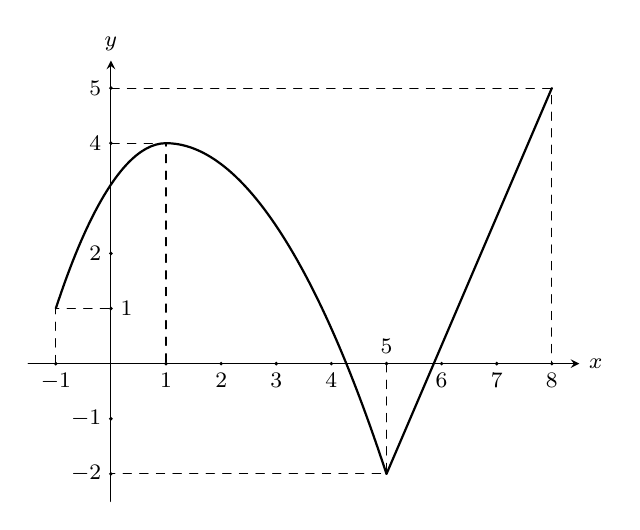
\begin{tikzpicture}[font=\footnotesize, line cap=round, line join =round, >=stealth, scale= .7]
			\def\xmin{-1}
			\def\xmax{8}
			\def\ymin{-2}
			\def\ymax{5}
			\draw[-stealth] (\xmin-.5,0)--(\xmax+.5,0)node[right]{$x$};
			\draw[-stealth] (0,\ymin-.5)--(0,\ymax+.5)node[above]{$y$};
%			\draw[thick,smooth, samples=200] plot[domain=-1:5] (\x,{(-1/2*(\x)^2+(3/2)*(\x)+3)});
			\draw[thick,smooth, samples=200] (-1,1) parabola bend (1,4) (5,-2);
			\draw[thick] (5,-2)--(8,5);
			\foreach \x in {-1,1,2,3,4,6,7,8}
			\fill[black] (\x,0) circle (1pt)node[below]{$\x$};
			\foreach \x in {5}
			\fill[black] (\x,0) circle (1pt)node[above]{$\x$};
			\foreach \y in {-2,-1,2,4,5}
			\fill[black] (0,\y) circle (1pt)node[left]{$\y$};
			\foreach \y in {1}
			\fill[black] (0,\y) circle (1pt)node[right]{$\y$};
			\draw[dashed]
			(-1,0)--(-1,1)--(0,1)
			(0,4)--(1,4)--(1,0)
			(5,0)--(5,-2)--(0,-2)
			(0,5)--(8,5)--(8,0)
			;
		\end{tikzpicture}
	\end{center}
\loigiai 
{
Hàm số đồng biến trên các khoảng $(-1;1)$, $(5;8)$ và nghịch biến trên khoảng $(1;5)$.\\
Tập giá trị của hàm số trên đoạn $[-1;8]$ là $[-2;5]$.
}
\end{bt}
\begin{bt}%[0T3K2-1]%[Dự án đề kiểm tra HKII NH22-23- Nguyễn Cường]%[THPT Trưng Vương]
	Tìm $m$ để hàm số $y=(2m+1)x^2-5mx+m+2$ có giá trị nhỏ nhất bằng $ -1 $.\\
	\dapso $m = 2$.
	\loigiai 
	{
	\begin{itemize}
		\item Xét $2m+1=0\Leftrightarrow m=-\dfrac{1}{2}$, khi đó hàm số trở thành $y=\dfrac{5}{2}x+\dfrac{3}{2}$ nên không có giá trị nhỏ nhất.
		\item Xét $2m+1\ne 0\Leftrightarrow m\ne -\dfrac{1}{2}$. Khi đó đồ thị hàm số là một đường parabol có tọa độ đỉnh là $I\left(\dfrac{5m}{4m+2};\dfrac{-17m^2+20m+8}{8m+4}\right)$.\\
		Giá trị nhỏ nhất của hàm số bằng $-1$ khi và chỉ khi
		\allowdisplaybreaks
		\begin{eqnarray*}
			&&\heva{&2m+1>0\\&\dfrac{-17m^2+20m+8}{8m+4}=-1}\\
			&\Leftrightarrow&\heva{&m>-\dfrac{1}{2}\\&-17m^2+20m+8=-8m-4}\\
			&\Leftrightarrow&\heva{&m>-\dfrac{1}{2}\\&-17m^2+28m+12=0}\\
			&\Leftrightarrow&\heva{&m>-\dfrac{1}{2}\\&\hoac{&m=2\quad \text{(Nhận)}\\&m=-\dfrac{6}{17}\quad \text{(Loại)}.}}
		\end{eqnarray*}
	\end{itemize}
Vậy $m=2$.
}
\end{bt}
\begin{bt}%[0T3B2-2]%[Dự án đề kiểm tra HKII NH22-23- Nguyễn Cường]%[THPT Trưng Vương]
	Tìm công thức hàm số bậc hai biết đồ thị hàm số có trục đối xứng là đường thẳng $x=2$, cắt trục tung tại điểm có tung độ bằng $ 3 $ và một trong hai giao điểm với trục hoành có hoành độ là $ 5 $.\\
	\dapso $y=\dfrac{-3}{5}x^2+\dfrac{12}{5}+3$.
	\loigiai 
	{
Xét hàm số $y=ax^2+bx+c$ với $a\ne 0$.\\
Ta có $\heva{&x=-\dfrac{-b}{2a}\\&x=0;y=3\\&x=5;y=0}\Leftrightarrow\heva{&\dfrac{-b}{2a}=2\\&c=3\\&25a+5b+c=0}\Leftrightarrow \heva{&4a+b=0\\&c=3\\&25a+5b+c=0}\Leftrightarrow\heva{&a=-\dfrac{3}{5}\\&b=\dfrac{12}{5}\\&c=3.}$\\
Vậy hàm số cần tìm là $y=\dfrac{-3}{5}x^2+\dfrac{12}{5}+3$.
}
\end{bt}


\begin{bt}%[0D6B4-2]%[VU Ngoc Hao-THPT-TRUNGVUONG-HKI-NH22-23]
	Kết quả nhảy xa (đơn vị: mét) của hai bạn An và Bình sau 5 lần được thống kê ở bảng dưới đây:
	\begin{center}
		\begin{tabular}{|c|c|c|c|c|c|}
			\hline
			An & $2{,}4$ & $2{,}6$ & $2{,}3$ & $2{,}5$ & $2{,}7$\\
			\hline
			Bình & $2{,}4$ & $2{,}5$ & $2{,}5$ & $2{,}5$ & $2{,}6$\\
			\hline
		\end{tabular}
	\end{center}
	\begin{enumerate}
		\item Kết quả trung bình của hai bạn có bằng nhau hay không?
		\item Tính phương sai và độ lệch chuẩn của mẫu số liệu thống kê kết quả 5 lần nhảy xa của mỗi bạn. Từ đó cho biết bạn nào có kết quả nhảy xa ổn định hơn.
	\end{enumerate}
%	\dapso a) Bằng nhau; b) $s_A^2 = \dfrac{1}{50}$; $s_B^2 = \dfrac{1}{250}$; $\sigma_A=\dfrac{1}{5\sqrt{2}}$; $\sigma_B=\dfrac{1}{5\sqrt{10}}$.
	\loigiai{
	\begin{enumerate}
		\item Ta có kết quả trung bình của An là 
		$$\bar{x}_A=\dfrac{2{,}4+2{,}6+2{,}3+2{,}5+2{,}7}{5}=2{,}5.$$
		 Kết quả trung bình của Bình là 
		 $$\bar{x}_B=\dfrac{2{,}4+2{,}5+2{,}5+2{,}5+2{,}6}{5}=2{,}5.$$
		 Vậy kết quả trung bình của hai bạn bằng nhau.
		\item Phương sai kết quả nhảy xa của An là 
		$$s_A^2 
		=\dfrac{(2{,}4-2{,}5)^2+(2{,}6-2{,}5)^2+(2{,}3-2{,}5)^2+(2{,}5-2{,}5)^2+(2{,}7-2{,}5)^2}{5}=
		 \dfrac{1}{50}.$$
		Độ lệch chuẩn kết quả nhảy xa của An là 
		$$\sigma_A=\sqrt{s_A^2}=\dfrac{1}{5\sqrt{2}}.$$
		Phương sai kết quả nhảy xa của Bình là 
		$$s_B^2 
		=\dfrac{(2{,}4-2{,}5)^2+(2{,}5-2{,}5)^2+(2{,}5-2{,}5)^2+(2{,}5-2{,}5)^2+(2{,}6-2{,}5)^2}{5}=
		 \dfrac{1}{250}.$$
			Độ lệch chuẩn kết quả nhảy xa của Bình là 
		$$\sigma_B=\sqrt{s_B^2}=\dfrac{1}{5\sqrt{10}}.$$
		Do $\sigma_B<\sigma_A$ nên kết quả nhảy xa của Bình ổn định hơn.
	\end{enumerate}
}
\end{bt}
\begin{bt}%[0H5B2-2]%[VU Ngoc Hao-THPT-TRUNGVUONG-HKI-NH22-23]
	Cho tứ giác $ABCD$, gọi $M$, $N$ lần lượt là trung điểm của $AB$, $CD$. Chứng minh rằng
	\begin{multicols}{2}
		\begin{enumerate}
			\item $\vv{AB}+\vv{DC}=\vv{AC}+\vv{DB}$.
			\item $\vv{BC}+\vv{AD}=2\vv{MN}$.
		\end{enumerate}
	\end{multicols}
	\loigiai{
		\begin{center}
			\begin{tikzpicture}[scale=1, font=\footnotesize, line join=round, 
			line cap=round, >=stealth]
				\path 
				(0.8,3) coordinate (A)
				(0,0) coordinate (B)
				(4,0) coordinate (C)
				(3,4) coordinate (D)
				($(A)!0.5!(B)$) coordinate (M)
				($(C)!0.5!(D)$) coordinate (N)
				;
				
				\draw (A)--(B)--(C)--(D)--cycle (M)--(N);
				
				\foreach \p/\r in {A/90,B/-120,C/-60,D/80,M/180,N/0}
				\fill (\p) circle (1.5pt) node[shift={(\r:3mm)}]{$\p$};
			\end{tikzpicture}
		\end{center}
	\begin{enumerate}
		\item Ta có VT=$\vv{AB}+\vv{DC}=\vv{AC}+\vv{CB}+\vv{DB}+\vv{BC}=
		\vv{AC}+\vv{DB}+\vv{CB}+\vv{BC}=\vv{AC}+\vv{DB}$=VP.
		\item Ta có 
	\[	\begin{aligned}
			VT=\vv{BC}+\vv{AD}=&\vv{BM}+\vv{MN}+\vv{NC}+\vv{AM}+\vv{MN}
			+\vv{ND}\\
			=&2\vv{MN}+(\vv{BM}+\vv{AM})+(\vv{NC}+\vv{ND})\\
			=&2\vv{MN}=VP.
		\end{aligned}\]
	\end{enumerate}
}
\end{bt}
\begin{bt}%[0H5B4-1]%[VU Ngoc Hao-THPT-TRUNGVUONG-HKI-NH22-23]
	Cho tam giác đều $ABC$ có cạnh bằng $a$.
	\begin{enumerate}
		\item Hãy tính độ dài của các véc-tơ sau: $\vv{AB}-\vv{AC}$; $\vv{AB}+\vv{AC}$.
		\item Cho $E$ là trung điểm của $AC$, hãy tính các tích vô hướng: $\vv{AB}\cdot\vv{AC}$; $\vv{BA}\cdot\vv{EB}$.
	\end{enumerate}
%	\dapso a) $a$, $a\sqrt{3}$; b) $\dfrac{a^2}{2}$, $\dfrac{-3a^2}{4}$.
	\loigiai{
		\begin{center}
			\begin{tikzpicture}[scale=1, font=\footnotesize, line join=round, 
			line cap=round, >=stealth]
				\path 
				(2,3) coordinate (A)
				(0,0) coordinate (B)
				(4,0) coordinate (C)
				($(C)!0.5!(B)$) coordinate (M)
				($(C)!0.5!(A)$) coordinate (E)
				;
				
				\draw (A)--(B)--(C)--cycle (A)--(M)(B)--(E);
				
				\foreach \p/\r in {A/90,B/-120,C/-60,M/-90,E/0}
				\fill (\p) circle (1.5pt) node[shift={(\r:3mm)}]{$\p$};
			\end{tikzpicture}
		\end{center}
		\begin{enumerate}
			\item Ta có $\left|\vv{AB}-\vv{AC}\right|=\left|\vv{CB}\right|=a.$\\
			$\left|\vv{AB}+\vv{AC}\right|=\left|2\vv{AM}\right|=2\cdot 
			\dfrac{a\sqrt{3}}{2}=a\sqrt{3}$ (với $M$ là trug điểm của $BC$).
			\item $\vv{AB}\cdot\vv{AC}=AB\cdot AC\cdot \cos60^\circ=a\cdot a\cdot \dfrac{1}{2}=\dfrac{a^2}{2}.$\\
			$\vv{BA}\cdot\vv{EB}=BA\cdot EB\cdot \cos150^\circ=a\cdot \dfrac{a\sqrt{3}}{2}\cdot \left(\dfrac{-\sqrt{3}}{2}\right)=-\dfrac{3a^2}{4}.$\\
		\end{enumerate}
	}
\end{bt}